
% * Week 1. (Jul 27) Introduction and R boot camp (Rob & Souhaib)
%   - Lecture 1:  What is Business Analytics? Show case of R.
%   - Lab 1: R exercises
%   - Lecture 2: Introduction to R programming
% - R, Rstudio
% - Rmarkdown
% - Examples:
%     prediction: bulldozers
%     classification: see JWHAT
%     clustering
%   Business analytics vs data science vs statistics vs econometrics 
%   Venn diagrams



\documentclass[14pt]{beamer}
\usepackage{pgf,tikz,pgfpages,amsmath,bm,fancyvrb,animate}
\usepackage{graphicx,bera,booktabs,multicol}
\usepackage[australian]{babel}
\usepackage[utf8]{inputenc}
\usepackage{media9}

\usepackage{comment}
\usepackage{array}

\usepackage{verbatim}

\definecolor{Orange}{RGB}{255,140,0}
\long\def\TCorange#1{\textcolor{Orange}{#1}}
\long\def\TCblue#1{\textcolor{blue}{#1}}

\newcommand\Wider[2][3em]{%
\makebox[\linewidth][c]{%
  \begin{minipage}{\dimexpr\textwidth+#1\relax}
  \raggedright#2
  \end{minipage}%
  }%
}

\usetheme{Monash}
\def\ben{\begin{enumerate}[<+-| alert@+>]}
\def\een{\end{enumerate}}

%\AtBeginSubsection[]  
%  {  
%    \begin{frame}<*>{Outline}  
%      \tableofcontents[currentsection,currentsubsection]  
%    \end{frame}  
%  }


\graphicspath{{../figures/}}

\title[Introduction to Business Analytics and R]{Business Analytics}
\author{Week 1.\\ Introduction to Business Analytics \& R}
\date{27 July 2016}

\DefineShortVerb{\"}
\def\FancyVerbFormatCom{\color[rgb]{0.6,0,1}\relax}


\def\source#1{\vspace{-0.4cm}\par{\fontsize{6}{8}\sffamily \url{#1}}}
\def\inlinesource#1{\hbox{\fontsize{6}{8}\sffamily \url{#1}}}

 
\begin{document}

\begin{frame}[plain]{}
\maketitle
\begin{textblock}{11}(0.5,1.3){\color{white}\large
\textbf{ETC3250}}
\end{textblock}


\end{frame}

	
\begin{frame}{Who are we?}\Large

\begin{tabular}{l >{\centering\arraybackslash}m{3in}}
\raisebox{-1cm}{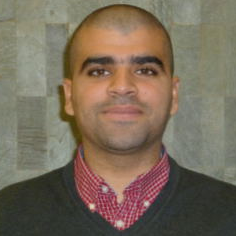
\includegraphics[width=2.5cm]{souhaib-new}} & Souhaib BenTaieb (Chief examiner) \\
\raisebox{-1cm}{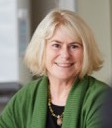
\includegraphics[width=2.5cm]{di}}& Di Cook (Co-lecturer)   \\
\raisebox{-1cm}{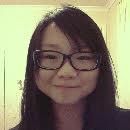
\includegraphics[width=2.5cm]{shin}}& Shin Tan (Teaching Associate)
\end{tabular}

\end{frame}


\begin{frame}{Outline}\fontsize{11}{14}\sf\tabcolsep=0.1cm
\centerline{\begin{tabular}{rlll}
\hline
\bf Week& \textbf{Topic} & \bf Chapter & \bf Lecturer\\
\hline
1  & Introduction to business analytics \& R     & 1    & Souhaib   \\
2  & Statistical learning                        & 2    & Souhaib\\
3  & Regression for prediction                   & 3    & Souhaib \\
4  & Resampling                                  & 5    & Souhaib \\
5  & Dimension reduction                         & 6,10 & Souhaib\\
6  & Visualization                               &      & Di \\
7  & Visualization                               &      & Di \\
8  & Classification                              & 4,8  & Di \\
9  & Classification                              & 4,9  & Di \\
   &  & & \\
10 & Advanced classification                     & 8    & Souhaib \\
11 & Advanced regression                         & 6    & Souhaib\\
12 & Clustering                                  & 10   & Souhaib
\end{tabular}}
\end{frame}

\begin{frame}{Assessment}

\begin{itemize}
\item Final exam (Open book) (3 hours): 60\%
\item One project due at the end of the semester: 20\%
\item Ten short weekly assignments: 15\% (1.5\% each)
\item Class exercises: 5\%
\end{itemize}

\begin{block}{}{\tabcolsep=0.1cm\begin{tabular}{lll}
  \textbf{Task}     & \textbf{Due Date}     & \textbf{Value} \\ \midrule
    Final exam        & Official exam period  & 60\%    \\
    Project           & Fri 23 October        & 20\%           \\      
      Assignments 1--10 & Day after the lab 11:55pm & 15\% \\
  Class exercises & End of selected class & 5\% 
\end{tabular}}
\end{block}

\end{frame}


\begin{frame}{Moodle site}

% \centerline{\begin{beamercolorbox}[wd=12cm,rounded=true,shadow=true]{block body alerted}
% \bf\Large\centering
% Moodle
% \end{beamercolorbox}}
\begin{itemize}
\item Includes all lecture notes, handouts, assignments
\item Forum for asking questions, etc.
\item No email please --- use the forum.
\item Assignment submissions
\end{itemize}

\end{frame}

\begin{frame}{Key reference}\large

\begin{block}{}\bf
{James, Witten, Hastie and Tibshirani (2012) \emph{An Introduction to Statistical Learning}. Springer.}
\end{block}
\begin{alertblock}{}\Large
\centerline{\bf www.statlearning.com}
\end{alertblock}

\begin{itemize}
\item Free pdf online
\item Data sets in associated R package \textbf{ISLR}
\item R code for examples
\end{itemize}
\end{frame}


\begin{frame}{What is business analytics?}

%Using \textbf{data} to gain \textbf{insights} and \textbf{understanding} of business problems and performance.

\begin{block}{}
``\emph{Business analytics} is the \textbf{scientific process} of transforming \textbf{data} into \textbf{insight} for making better \textbf{decisions}''
\end{block}\pause
\begin{itemize}
\item \textbf{Broader than \TCblue{business intelligence}} which focuses on describing and predicting performance.
\item \textbf{Broader than \TCblue{econometrics}} as we are interested in more than economics and  finance.
\item \textbf{Narrower than \TCblue{data science}} as we are focusing on {business issues}.
\end{itemize}

\end{frame}



\begin{frame}{What is business analytics?}

\centering{\includegraphics[width = \linewidth]{spectrum-analytics}}

\end{frame}

\begin{frame}{What is business analytics?}

{\small
\begin{itemize}
	\item Financial Analytics
	\item Human Resource Analytics	
	\item Marketing Analytics
	\item Health Care Analytics
	\item Supply Chain Analytics
	\item Analytics for Government and Nonprofits
	\item Sport Analytics
	\item Web Analytics
\end{itemize}
}

\end{frame}



\begin{frame}{Related fields}\fontsize{12}{12}\sf
\begin{block}{}
``\TCblue{Statistics} is the \textbf{science of learning from \underline{data}}, and of \textbf{measuring}, \textbf{controlling}, and \textbf{communicating \TCorange{uncertainty}}; [...]''.
\end{block}\pause

\begin{block}{}
``\TCblue{Machine learning} is a \textbf{scientific discipline} that explores the \textbf{construction and study of \TCorange{algorithms}} that can \textbf{learn from \underline{data}}''.
\end{block}\pause

\begin{block}{}
``\TCblue{Data mining}, [...], is the \textbf{computational process} of \textbf{discovering \TCorange{patterns}} in \textbf{large \underline{data} sets} involving methods at the intersection of \textbf{artificial intelligence}, \textbf{machine learning}, \textbf{statistics}, and \textbf{database systems}''.
\end{block}\pause

\begin{block}{}
``\TCblue{Data Science} means the \textbf{\TCorange{scientific study}} of the \textbf{creation}, \textbf{validation} and \textbf{transformation of \underline{data}} to \textbf{\TCorange{create meaning}}''.
\end{block}

\end{frame}


\begin{frame}{Why study business analytics?}
\vspace{-.3cm}
\begin{center}
\includemedia[
label=obama_data_science,
%  width=0.4\linewidth,
%  height=0.3\linewidth,
%  width=0.6\linewidth,height=0.3375\linewidth,
%  width=0.9\linewidth,height=0.5\linewidth,
  width=.99\linewidth,height=0.55\linewidth,
%   width=0.8\linewidth,height=0.45\linewidth,
  activate=pageopen,
  addresource=videos/obama-datascience.mp4,
  flashvars={source=videos/obama-datascience.mp4
&modestbranding=1 % no YT logo in control bar
&autohide=1 % controlbar autohide
&showinfo=0 % no title and other info before start
&rel=0
  }
]{}{VPlayer.swf}
\mediabutton[
mediacommand=obama_data_science:playPause,
overface=\color{blue}{\fbox{\strut Play/Pause}},
downface=\color{red}{\fbox{\strut Play/Pause}}
]{\fbox{\strut Play/Pause}} 
%\quad {\small Source: \url{https://www.youtube.com/watch?v=vbb-AjiXyh0}}
\end{center}


%false discoveries / wrong conclusions from data

\end{frame}


\begin{frame}{Why study business analytics?}
\vspace{-.3cm}
\begin{center}
\includemedia[
label=rob,
  width=.99\linewidth,height=0.55\linewidth,
  activate=pageopen,
  addresource=videos/rob.mp4,
  flashvars={source=videos/rob.mp4
&modestbranding=1 % no YT logo in control bar
&autohide=1 % controlbar autohide
&showinfo=0 % no title and other info before start
&rel=0
  }
]{}{VPlayer.swf}
\mediabutton[
mediacommand=rob:playPause,
overface=\color{blue}{\fbox{\strut Play/Pause}},
downface=\color{red}{\fbox{\strut Play/Pause}}
]{\fbox{\strut Play/Pause}} 
%\quad {\small Source: \url{https://www.youtube.com/watch?v=vbb-AjiXyh0}}
\end{center}


\end{frame}


\begin{frame}{Some quotes}
\begin{alertblock}{}
By 2018, the US could face a shortage of up to 190.000 workers with analytical skills ---McKinsey
\end{alertblock}

\begin{block}{Top-ranked jobs 2015: CareerCast}
\fontsize{10}{10}\sf
\begin{enumerate}
\item \only<1>{\alert}{Actuary} 
\item Audiologist  
\item \only<1>{\alert}{Mathematician}  
\item \only<1>{\alert}{Statistician}  
\item Biomedical Engineer  
\item \only<1>{\alert}{Data Scientist}  
\item Dental Hygienist 
\item Software Engineer 
\item Occupational Therapist 
\item Computer Systems Analyst 
\end{enumerate}
\end{block}



\end{frame}

\begin{frame}{Some quotes}
\begin{alertblock}{}
By 2018, the US could face a shortage of up to 190.000 workers with analytical skills ---McKinsey
\end{alertblock}


\begin{block}{Top-ranked jobs 2016: CareerCast}
\fontsize{10}{10}\sf
\begin{enumerate}
\item \only<1>{\alert}{Data Scientist}
\item \only<1>{\alert}{Statistician}
\item Information Security Analyst
\item Audiologist
\item Diagnostic Medical Sonographer
\item \only<1>{\alert}{Mathematician}
\item Software Engineer
\item Computer Systems Analyst
\item Speech Pathologist
\item \only<1>{\alert}{Actuary}
\end{enumerate}
\end{block}


\end{frame}

\begin{frame}{Some quotes}

\small
\begin{block}{}
\textit{\textbf{\TCblue{Data Scientist}: The Sexiest Job of the 21st Century}} ---  Thomas H. Davenport and D. J. Patil, Harvard Business Review, October 2012.
\end{block}

\begin{block}{}
\textit{\textbf{To have any hope of extracting anything useful from big data, … effective inferential skills are vital. That is, at the heart of extracting value from big data lies \TCblue{statistics}} --- David J. Hand, 2014.}
\end{block}


\begin{block}{}
\textit{\textbf{Most of my life I went to parties and heard a little groan when people heard what I did. Now they are all excited to meet me} ---  Robert Tibshirani, a \TCblue{statistics} professor at Stanford University, New York Times, January 26, 2012.}
\end{block}

\end{frame}



\begin{frame}{Am I a data scientist?}\fontsize{12}{14}\sffamily


\begin{block}{April 2013: Larry Wasserman blog}
\textbf{Data science: the end of statistics?}

\textit{If you're analyzing data, you're doing statistics. You can call it data science or informatics or analytics or whatever, but it's still statistics.} \hfill\inlinesource{normaldeviate.wordpress.com/2013/04/13/data-science-the-end-of-statistics/}
\end{block}




\only<2->{\begin{block}{April 2013: Karl Broman blog}

\textbf{Data science is statistics}

\textit{You may not like what some statisticians do. You may feel they don't share your values. They may embarrass you. But that shouldn't lead us to abandon the term “statistics”.}

\mbox{}\hfill
\inlinesource{kbroman.wordpress.com/2013/04/05/data-science-is-statistics/}

\end{block}}

\only<3>{\begin{block}{July 2013: ASA President blog}
Davidian: \textbf{Aren't \emph{we} data science?}
\end{block}}

\vspace*{10cm}

\end{frame}

\begin{frame}{Am I a data scientist?}\fontsize{12.5}{15}\sffamily


\begin{alertblock}{November 2013: Andrew Gelman blog}
\textbf{Statistics is the \emph{least} important part of data science}\parskip=.5ex

\textit{There’s so much that goes on with data that is about computing, not statistics. I do think it would be fair to consider statistics as a subset of data science \dots}

\textit{Statistics is important—don’t get me wrong—statistics helps us correct biases \dots\ estimate causal effects \dots\  regularize so that we’re not overwhelmed by noise \dots\ fit models \dots\ visualize data \dots\ I love statistics! But it’s not the most important part of data science, or even close.}
\hfill\inlinesource{andrewgelman.com/2013/11/14/statistics-least-important-part-data-science/}
\end{alertblock}

\vspace*{10cm}

\end{frame}




\begin{frame}{Am I a data scientist?}
\placefig{0.1}{1.0}{height=8.3cm}{Data_Science_VD}
\only<2>{\begin{textblock}{4.8}(7.6,4.9)\begin{block}{}\fontsize{12}{14}\sffamily A data scientist is someone who is better at statistics than any software engineer and better at software engineering than any statistician.\end{block}\end{textblock}}

\begin{textblock}{12.8}(0.1,9.)\fontsize{5}{7}\sffamily
Source: Drew Conway, Sept 2010.  \url{drewconway.com/zia/2013/3/26/the-data-science-venn-diagram.} Reproduced under a Creative Commons License.
\end{textblock}
\end{frame}


\begin{frame}{Am I a data scientist?}\vspace*{-0.2cm}
\centerline{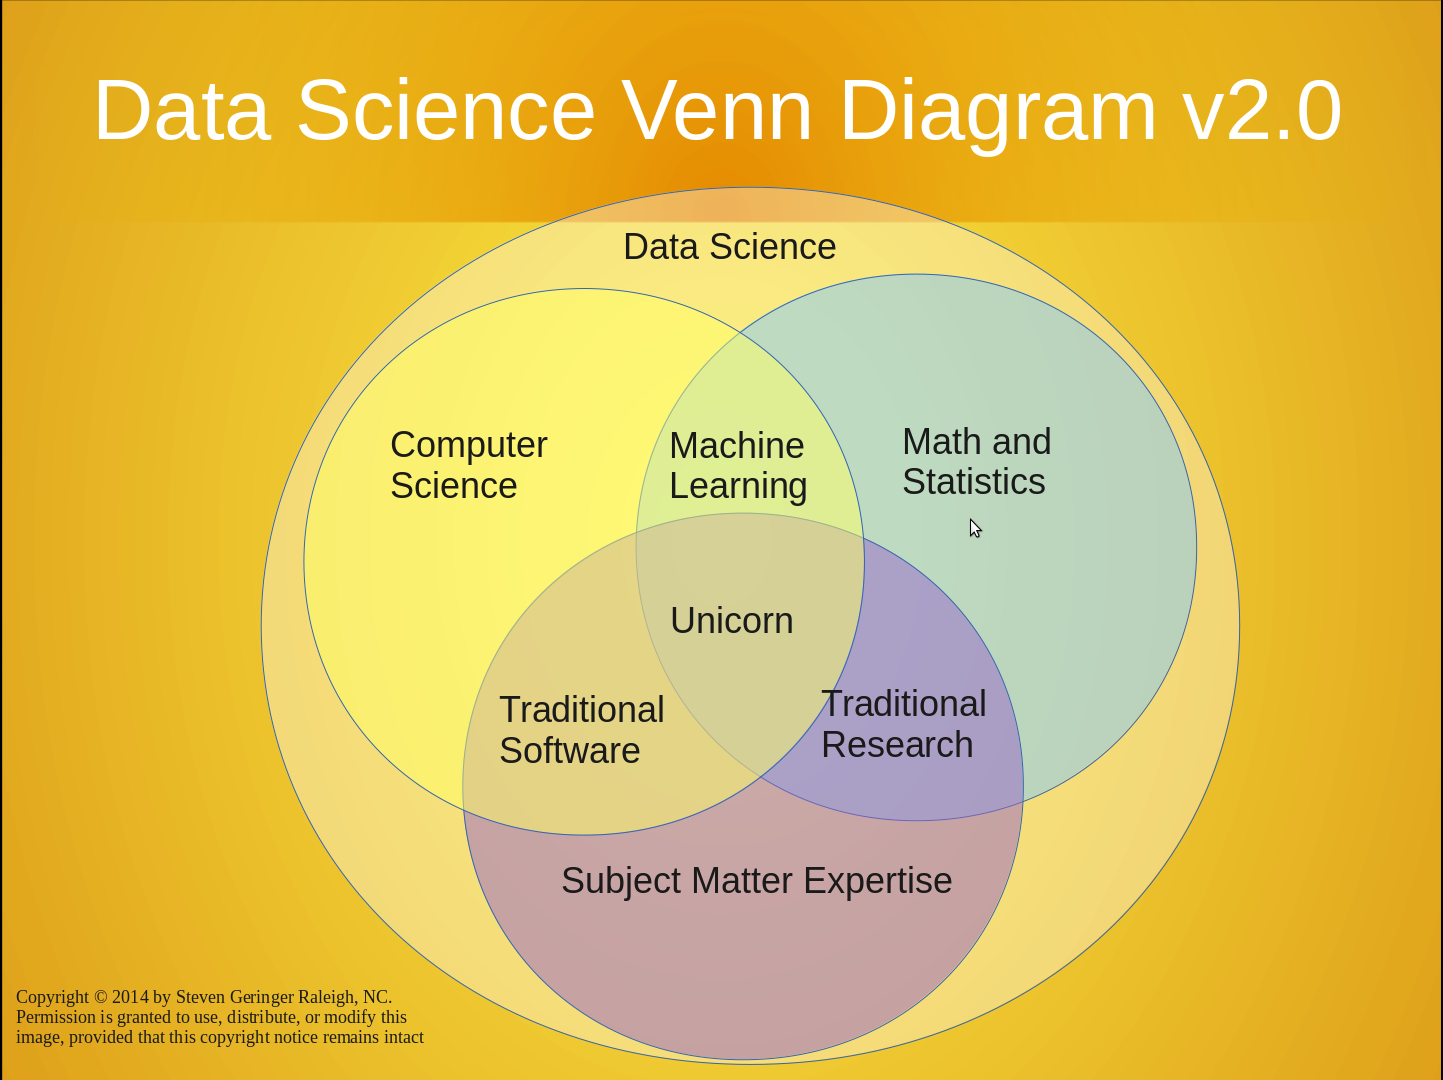
\includegraphics[height=8.2cm]{Venn-Diagram-of-Data-Scientist-Skills-}}
\end{frame}

\begin{frame}{\large The business analytics process}

\centerline{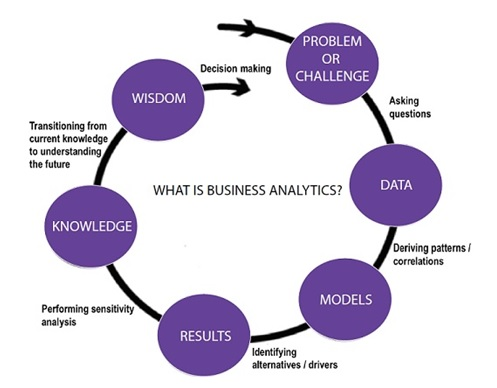
\includegraphics[height=8.2cm]{BAprocess}}

\begin{textblock}{12.8}(0.1,9.)\fontsize{5}{7}\sffamily
Source: \url{http://www.stern.nyu.edu/programs-admissions/executive-education/short-courses/schedule/short-course-program-7}
\end{textblock}

\end{frame}


\begin{frame}{\large The business analytics tools}
\begin{itemize}
\item Pulling together and cleaning data
\item  Exploring and visualizing data
\item  Fitting, comparing and assessing models
\item  Tools for fitting models: optimization, training and testing
\item  Tools for understanding randomness: simulation, resampling, permutation, cross-validation
\item Tools for handling large data sets: dimension reduction, regularization, distributed computing.
\end{itemize}
\end{frame}

\begin{frame}{Learning goals}\fontsize{13}{14}\sf

\begin{enumerate}
\item Select and develop appropriate models for clustering, prediction or classification
\item Estimate and simulate from a variety of statistical models, and measure the uncertainty of a prediction or classification using resampling methods
\item Apply business analytic tools to produce innovative solutions in finance, marketing, economics and related areas
\item Manage very large data sets in a modern software environment, and explain and interpret the analyses undertaken clearly and effectively.
\end{enumerate}

\pause

\begin{alertblock}{Teaching and learning approach}
Two 1-hour lectures and a one 1.5 hour lab class each week for 12 weeks.
\end{alertblock}
\end{frame}

\begin{frame}{R}
 

\placefig{.4}{1.2}{width=6cm}{Rlogo}

\only<2>{\placefig{7}{3.5}{width=5.5cm}{RStudio-Ball}
\begin{textblock}{5.5}(7,3)\centerline{\structure{RStudio}}\end{textblock}}
\end{frame}


\end{document}


%\input{temp.tex}